\documentclass[11pt]{article}

% ----- Encoding -----
\usepackage[utf8]{inputenc}
% ----- Geometry -----
\usepackage{fullpage}
% ----- Language -----
\usepackage[american]{babel}
% ----- Math -----
\usepackage{amsmath}
\usepackage{mathtools}
% ----- Tables -----
\usepackage{tabularx}
\usepackage{booktabs}
% ----- Text -----
\usepackage{csquotes}
\usepackage{outlines}
% ----- Visuals -----
\usepackage{color}
\usepackage{graphicx}
\usepackage{tikz}
\usepackage{forest}

% ----- Document -----
% TODO: figure out where second correct goes?

\begin{document}

\section{Basic equations}

\subsection{Up-down PC equation}

For the up-down paradigm, we assume that the psychometric function takes a simple shape as in Dai and Micheyl (XXXX).

\begin{equation}
		\text{PC} = \frac{1}{2} \lambda + (1 - \lambda) \Phi \left(\frac{1}{\sqrt{2}} d' \right)
\end{equation}

\begin{itemize}
	\item PC = proportion of correct responses
	\item $\lambda$ = Controls inattention... $\lambda=0$ implies complete attention to task, $\lambda=1$ implies complete inattention to task
	\item $d'$ = Sensitivity, $d'=1$ implies 76.0\% correct, $d'=2$ implies 92.1\% correct
\end{itemize}

\begin{equation}
		d' = \frac{\log_{10}(f_2/f_1)}{\alpha}
\end{equation}

\begin{itemize}
	\item $f_2$, $f_1$ = frequencies of second and first tones in Hz\ldots note that here we implicitly assume that $f_2 > f_1$, but when $f_1 > f_2$ we simply sign-flip $d'$ (this is achieved in our code via the \texttt{second\_correct} variable)
	\item $\alpha$ = (inverse) constant of proportionality between log-transformed difference in frequency and sensitivity\ldots when $\log_{10}(f_2/f_1)$ is equal to $\alpha$, then $d'$ is 1 and percent correct should be 76.0\%\ldots essentially a measure of coding noise 
\end{itemize}

\subsection{Same-different PC equation}

For the same-different paradigm, we assume that a differencing approach is used to make decisions. That is, the listener estimates the difference of the two tones' frequenices and then decides to answer ``same'' or ``different'' based on whether that estimate falls within or beyond a decision region bouned by $[-\tau, \tau]$ (DeCarlo, 2013).
It follows then that\ldots 

\begin{equation}
		p(\text{``different''}|\text{Different}) = 1 - \Phi\left( \frac{d' + \tau}{\sqrt{2}} \right) + \Phi\left(\frac{d' -\tau}{\sqrt{2}} \right) 
\end{equation}

\begin{equation}
		p(\text{``same''}|\text{Same}) = \Phi\left( \frac{\tau}{\sqrt{2}} \right) - \Phi\left(\frac{-\tau}{\sqrt{2}} \right) 
\end{equation}

\section{Sensory bias equations}

In the sensory bias model, we assume that estimates of $f_1$ are biased in favor of the mean perceived frequency $\hat{f}_\text{mean}$. 
Thus, when the tones are high-low and are both below the mean, this produces an increase in performance (as the perceptual difference between the tones is ``enhanced'' by the bias). 
At the same time, when the tones are low-high and both below the mean, this produces a decrease in performance (as the perceptual difference between the tones is diminished by the bias). 
The converse is true for tones above the mean.
Notably, because this effect enters at the ``sensory'' stage into the equations via $d'$, it impacts performance estimates for both the up-down and the same-diff paradigms.

\subsection{Sensory bias up-down PC equation}

\begin{equation}
		\text{PC}_\text{sensory} = \frac{1}{2} \lambda + (1 - \lambda) \Phi \left(\frac{\log_{10}(f_2/\hat{f}_1)}{\sqrt{2}\alpha} \right)
\end{equation}

\begin{equation}
		\hat{f}_1 = \log_{10}(f_1) - \omega \left( \log_{10}(\hat{f}_\text{mean}) - \log_{10}(f_1) \right)
\end{equation}

\begin{itemize}
	\item $\hat{f}_1$ = Bayesian-like estimate of $f_1$, derived from weighted average of $f_1$ and $\hat{f}_\text{mean}$
	\item  $\hat{f}_\text{mean}$ = the perceived mean of the frequency range
	\item $\omega$ = parameter controlling weighting of true $f_1$ and perceived mean $\hat{f}_\text{mean}$ in calculation of $\hat{f}_1$
\end{itemize}

\subsection{Sensory bias same-diff PC equation}

\begin{equation}
		p(\text{``different''}|\text{Different})_\text{sensory} = 1 - \Phi\left( \frac{\frac{\log_{10}(f_2/\hat{f}_1)}{\alpha} + \tau}{\sqrt{2}} \right) + \Phi\left(\frac{\frac{\log_{10}(f_2/\hat{f}_1)}{\alpha} -\tau}{\sqrt{2}} \right) 
\end{equation}

\begin{equation}
		p(\text{``same''}|\text{Same})_\text{sensory} = \Phi\left( \frac{\tau}{\sqrt{2}} \right) - \Phi\left(\frac{-\tau}{\sqrt{2}} \right) 
\end{equation}

\section{Criterion shift equation}

In the criterion shift model, we assume that listeners are biased in their up-down responses as a function of the distance between the frequencies of the tone pair and the perceived mean of the frequency range.
Specifically, they are liable to respond ``up'' more often as the tone pair increases in frequency above the mean, which favors low-high pairs and disfavors high-low pairs (same as the sensory bias model).
In contrast, they are liable to response ``down'' more often as the tone pair decreases in frequency below the mean, which favors high-low pairs and disfavors low-high pairs (again, same as the sensory bias model). 
In the same-different task, listeners are assumed to not be impacted by the bias (because it is a \emph{response} bias based on the question ``up or down?'', which is not asked in the same-diff paradigm). 

\subsection{Criterion shift same-diff PC equation}

\begin{equation}
		\text{PC}_\text{criterion} = \frac{1}{2} \lambda + (1 - \lambda) \Phi \left(\frac{d'}{\sqrt{2}} + k\right)
\end{equation}

\begin{equation}
		k = s \left( \sqrt{f_2 \times f_1} - \hat{f}_\text{mean} \right)
\end{equation}

\begin{itemize}
	\item $k$ = size of criterion shift at a given $(f_1, f_2)$, is proportion to the difference between the geometric mean of $f_1$ and $f_2$ and the perceived mean of the frequency range $\hat{f}_\text{mean}$
	\item $s$ = constant of proportionality / slope of criterion shift
\end{itemize}

\begin{figure}
	\centering
	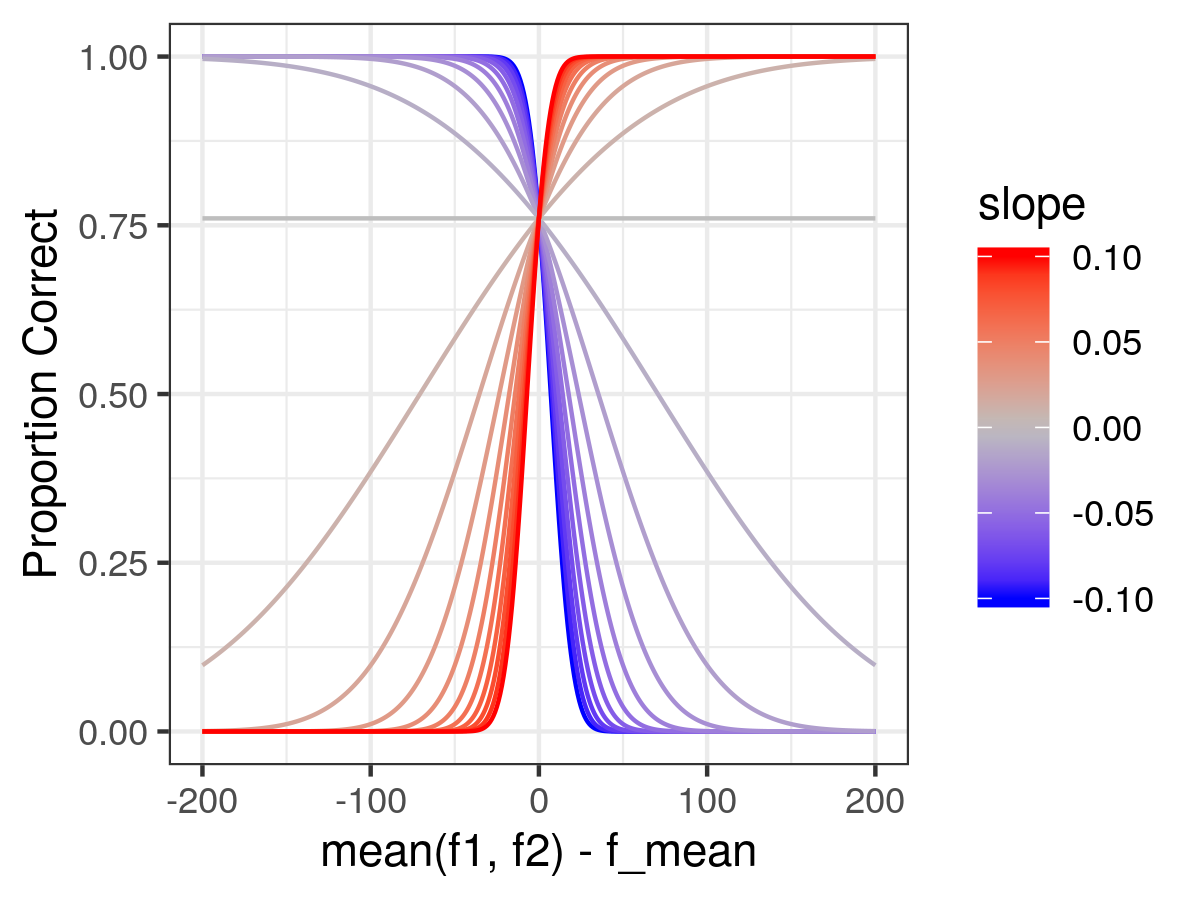
\includegraphics{slope}
\end{figure}

Note that we implicitly assume here than $f_2 > f_1$, when this is not true, both the sign of $d'$ and the sign of $k$ are flipped. 

\subsection{Criterion shift up-down PC equation}

\begin{equation}
		p(\text{``different''}|\text{Different}) = 1 - \Phi\left( \frac{d' + \tau}{\sqrt{2}} \right) + \Phi\left(\frac{d' -\tau}{\sqrt{2}} \right) 
\end{equation}

\begin{equation}
		p(\text{``same''}|\text{Same}) = \Phi\left( \frac{\tau}{\sqrt{2}} \right) - \Phi\left(\frac{-\tau}{\sqrt{2}} \right) 
\end{equation}

\end{document}
